\documentclass[journal]{vgtc}                % final (journal style)
%\documentclass[review,journal]{vgtc}         % review (journal style)
%\documentclass[widereview]{vgtc}             % wide-spaced review
%\documentclass[preprint,journal]{vgtc}       % preprint (journal style)

%% Uncomment one of the lines above depending on where your paper is
%% in the conference process. ``review'' and ``widereview'' are for review
%% submission, ``preprint'' is for pre-publication, and the final version
%% doesn't use a specific qualifier.

%% These few lines make a distinction between latex and pdflatex calls and they
%% bring in essential packages for graphics and font handling.
%% Note that due to the \DeclareGraphicsExtensions{} call it is no longer necessary
%% to provide the the path and extension of a graphics file:
%% 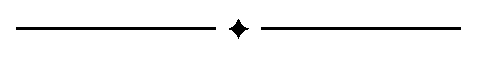
\includegraphics{diamondrule} is completely sufficient.
%%
\ifpdf%                                % if we use pdflatex
  \pdfoutput=1\relax                   % create PDFs from pdfLaTeX
  \pdfcompresslevel=9                  % PDF Compression
  \pdfoptionpdfminorversion=7          % create PDF 1.7
  \ExecuteOptions{pdftex}
  \usepackage{graphicx}                % allow us to embed graphics files
  \DeclareGraphicsExtensions{.pdf,.png,.jpg,.jpeg} % for pdflatex we expect .pdf, .png, or .jpg files
\else%                                 % else we use pure latex
  \ExecuteOptions{dvips}
  \usepackage{graphicx}                % allow us to embed graphics files
  \DeclareGraphicsExtensions{.eps}     % for pure latex we expect eps files
\fi%

%% it is recomended to use ``\autoref{sec:bla}'' instead of ``Fig.~\ref{sec:bla}''
\graphicspath{{figures/}{pictures/}{images/}{./}} % where to search for the images

\usepackage{microtype}                 % use micro-typography (slightly more compact, better to read)
\PassOptionsToPackage{warn}{textcomp}  % to address font issues with \textrightarrow
\usepackage{textcomp}                  % use better special symbols
\usepackage{mathptmx}                  % use matching math font
\usepackage{times}                     % we use Times as the main font
\renewcommand*\ttdefault{txtt}         % a nicer typewriter font
\usepackage{cite}

%% If you are submitting a paper to a conference for review with a double
%% blind reviewing process, please replace the value ``0'' below with your
%% OnlineID. Otherwise, you may safely leave it at ``0''.
\onlineid{0}

%% declare the category of your paper, only shown in review mode
\vgtccategory{Research}

%% Paper title - 1 pt for descriptive title
\title{The title for your project.}

%% This is how authors are specified in the journal style

%% indicate IEEE Member or Student Member in form indicated below
%% 1 pt for name
\author{Your Name Here}
\authorfooter{
%% insert punctuation at end of each item
\item
 Your Name is a graduate student at the University of Arizona. E-mail:[your
 NetID]@email.arizona.edu.
}

%other entries to be set up for journal
%\shortauthortitle{Firstauthor \MakeLowercase{\textit{et al.}}: Paper Title}

%% Abstract section - 5 pts
\abstract{
Abstract goes here. Summarize the project, why it is important, what you
plan to do, and what the community may learn from this in 150-250 words.

} % end of abstract

%% Keywords that describe your work. Will show as 'Index Terms' in journal
%% please capitalize first letter and insert punctuation after last keyword
%\keywords{Radiosity, global illumination, constant time}

%% ACM Computing Classification System (CCS). 
%% See <http://www.acm.org/class/1998/> for details.
%% The ``\CCScat'' command takes four arguments.

%\CCScatlist{ % not used in journal version
% \CCScat{K.6.1}{Management of Computing and Information Systems}%
%{Project and People Management}{Life Cycle};
% \CCScat{K.7.m}{The Computing Profession}{Miscellaneous}{Ethics}
%}

%% Uncomment below to include a teaser figure.
%   \teaser{
%   \centering
%   \includegraphics[width=16cm]{CypressView}
%   \caption{In the Clouds: Vancouver from Cypress Mountain.}
%  }

%% Uncomment below to disable the manuscript note
%\renewcommand{\manuscriptnotetxt}{}

%% Copyright space is enabled by default as required by guidelines.
%% It is disabled by the 'review' option or via the following command:
% \nocopyrightspace

\vgtcinsertpkg

%%%%%%%%%%%%%%%%%%%%%%%%%%%%%%%%%%%%%%%%%%%%%%%%%%%%%%%%%%%%%%%%
%%%%%%%%%%%%%%%%%%%%%% START OF THE PAPER %%%%%%%%%%%%%%%%%%%%%%
%%%%%%%%%%%%%%%%%%%%%%%%%%%%%%%%%%%%%%%%%%%%%%%%%%%%%%%%%%%%%%%%%

\begin{document}

%% The ``\maketitle'' command must be the first command after the
%% ``\begin{document}'' command. It prepares and prints the title block.

%% the only exception to this rule is the \firstsection command
\firstsection{Introduction} % or "Motivation"

\maketitle

% Introduction and/or Motivation - 15 pts

Strongly motivate your project in this section.

Summarize the problem you are trying to solve (or in other words, the question
you arre trying to answer).

Explain why the problem orr question is important -- who benefits from the
problem being solved or question being answered and in what way? If the
problem were to be solved or the question answered, what would that enable
people to do?

Summarize what you plan to do to solve the problem.

% You may want to end this section by summarizing it again as a list:
The aims of this research are:
\begin{itemize}
  \item the design of an evaluation of an octopi onthology visualization
    system,
  \item the results of that evaluation,
  \item reflection on the methodology used and guidelines for future
    evaluations on visualizations for domain-experts
\end{itemize}

 

% 10 pts
\section{Background}
\label{sec:background}

Expand on what the reader needs to know and understand if it necessary to
adequately describe the problem. This may include definitions of terms and
explanations related to the problem area trying to be solved. For example, if
you want to evaluate a visualization system for editing film, you may need to
explain what people editing film are trying to accomplish with the system.

This section should answer the question "What does someone unfamiliar with the
area need to know to understand this project?" Often times this section
focuses on the \textit{domain}. For example, a new visualization for biology
data will explain the type of biology data used, the terminology that will be
used to describe it, the people who use it, and what they hope to learn from
it. If there is no specific domain, the background section may describe
general terms about the data abstraction (e.g. "We define a graph $G = (V, E)$
as..."), common practices, or other information for visualization researchers
who are not as familiar with this problem in comparison to all the others. 

% 10 pts
\subsection{Related Work}
\label{sec:related}

Discuss the work related to your project---include other related projects,
systems, or experiments, whether they be from visualization, other computing
areas, or even outside of computing. There are likely related academic works
(journal and conference articles), but you can also cite websites, books, and
other sources of information.

Prominent related works should be included for this milestone with a more
broad listing in the next milestone. (If you do an in depth related work
section in this milestone, you will not be expect to do ``more'' for the next
one.) 

If you are proposing a literature review, this section must include a
discussion of what similar ones exist already and should tie into the
motivation. Is the existing one old enough to be missing many relevant
advances? Are the other ones focused on related but different areas? Is the
previous one too broad and you seek a narrow focus?

For example, if my project involves comparing tools to analyze performance
data of distributed systems, I might want to cite
Perfopticon~\cite{Moritz:2015:EuroVis}. If my project involves how to evaluate
the design of a new library to support creating new visualizations, I might
want to cite d3js~\cite{d3js}. Note here I am using keys such as
"Moritz:2015:EuroVis" for citations. These refer to the full definitions in
proposal.bib.

ACM Digital Library makes it easy to get bib files for proposal.bib and there
are guides online for citing things like books~\cite{ware:2004:IVP},
theses~\cite{levoy:1989:DSV}, journal articles~\cite{Lorensen:1987:MCA}, and
conference proceedings~\cite{Nielson:1991:TAD}. There's even a format for
miscellaneous references (misc) such as websites and libraries not associated
with a article.



\section{Research Plan} 
\label{sec:research}

% 35 pts for explanation here combined with timeline below

Re-state the problem you are trying to solve or question you are trying to
answer and then explain how you plan to solve/answer it. Is it evaluating a
visualization? Is it applying a human-centered technique from outside
visualization to your visualization design project? Is it running an
experiment to find out something about people? Is it synthesizing a large
body of literature? Is it something else?

Note this is a {\em plan}. The plan may change as you make discoveries during
your project. However, you must describe what your plan is assuming everything
goes as expected. If there are some parts of the plan where you could run into
difficulties, state what those difficulties are and what alternative measures
you could take should those difficulties arise.

You may refer to other sections so as not to repeat yourself -- for example,
referencing Section~\ref{sec:background}.

You may want to use figures to illustrate your point, such as
Figure~\ref{fig:sample}.

\begin{figure}[h]
 \centering % avoid the use of \begin{center}...\end{center} and use \centering instead (more compact)
 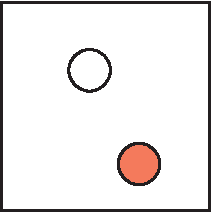
\includegraphics[width=1.5in]{figs/sample}
 \caption{Figure illustrating some proposed designs.}
 \label{fig:sample}
\end{figure}

% 10 pts
\subsection{Resources}
\label{sec:resources}

Describe any resources you need for this project here and whether or not you
already have access to them. If your project requires certain software, like
visualization systems to evaluate or survey software, do you have it? If not,
do you plan on writing it?

If your project needs data to visualization, describe whether you already have
access to the data and if not, what is required to obtain the data. If you
don't already have the data, explain how long it will take to retrieve it. 

If your project needs participants, how many do you foresee it needing, at
least for piloting? What kinds of skills must these people have? For example,
if you are working on a tool for analyzing octopi videos, does  it only make
sense to ask octopi experts?

The point of this section is to determine if you are prepared to do the
proposed work and if the milestones take into account these resources.

% 5 pts
\subsection{Technology}
\label{sec:tech}

Describe what if any technologies you intend to use (e.g., programming
languages, platforms, apps, existing libraries) and why they make sense for
your project. Do they serve your users better than other technologies? Are you
able to take advantage of existing work/libraries for your domain with this
technology rather than HTML/CSS/JS and d3js?  

\subsection{Timeline}
\label{sec:timeline}

Adapt the milestones for the class project to the specifics of your project
and summarize in Table~\ref{tab:milestones}. Do not simply copy the current
text as is. Your milestones should be specific to your problem.

The expectations are as follows:

\vspace{1.5ex}\noindent\textbf{Project Milestone Two} should include the
initial proposed methodology of any work you plan to do in detail, including
justification and rationale for why that methodology was chosen. It should
contain specifics of the design for your problem, such as how people will be
recruited, what they will be asked to do, and what artifacts need to be
generated, how the design is validated, and how results will be analyzed. Any
pre-studies/pilot work should also be in the plan.

If you are doing a literature review, you should have the methodology for how
you will find the literature and collect data based on it. For example, which
venues will you start with? What years? Keyword searches? What is your policy
for following citations?

No matter what kind of project you do, also compile an IRB proposal, including
all forms (e.g., F107), and consent documents. DO NOT submit it to the IRB, it
is for class use only. Do the proposal as if you were proposing Project
Milestone 2, unless you are doing a literature review. In that case, choose
one paper from your initial pool and fill out the IRB proposal as if you were
proposing that experiment.

Additionally, the related works should be updated with a more thorough
literature review. Changes to the status of the data and the choices of
technology should be discussed.

\vspace{1.5ex}\noindent\textbf{Project Milestone Three} should include
revisions following the project in-progress presentations as well as the
results of the first chunk of work that needs to be done. This first `chunk'
of work may involve implementation work (fixing interfaces, adding logging
features, creating visualizations for an experiment). Include images of these
implemented pieces and discussion of what they do. Demonstrations should run
with minimal effort and the code should be included in the repository.

Depending on needs, rather than coding, the chunk may involve piloting small
pieces of your design, decreasing factors in the study, or generating
experimental objects (e.g., more examples/trials/tutorials).

For projects involving heavy literature review, this milestone should include
annotations and notes for half of the selected papers.  Including a
preliminary schema for categorizing will help me give you feedback.

In the corresponding report, discussion of project progress as well as any
revisions to the data, methodology, technology choice, and scope should be
included.

\vspace{1.5ex}\noindent\textbf{Project Milestone Four} should include a
complete working prototype of the main project artifacts, such as the working
study with experimental objects and stimuli complete, the visualization tool
and evaluation script, or completed literature annotations with a
categorization scheme. The demonstration should run with minimal effort and
the code should be included in the repository.

If your project involves human participants directly, you should have also run
a pilot study by now with one or two volunteers. Report on the results of this
pilot---what worked? what didn't? what needs to be changed?

In the corresponding report, discussion of project progress as well as any
revisions to the data, technology choice, and scope should be included. The
plan for evaluation especially should be updated indicating the plan for
milestone five and any preliminary work in the design of that evaluation.


\vspace{1.5ex}\noindent\textbf{Project Milestone Five} should include the
final revisions of any study methodology, artifacts, or literature survey.
Additional pilots or study runs based on what was learned in the previous
milestone may be reported. If the study was run, analysis of the data
Artifacts generated (e.g., pre-observation plan, observation notes, data from
studies) during this study should be included in the repository.
Literature-based projects should include a refinement of the findings from the
previous milestone.

Additionally, this milestone should include reflection upon what was learned
in this project, with suggestions for people trying to do similar work.


\begin{table}[h]
%% Table captions on top in journal version
 \caption{Project Milestones}\vspace{1ex} % the \vspace adds some space after the top caption
 \label{tab:milestones}
 \scriptsize
 \centering % avoid the use of \begin{center}...\end{center} and use \centering instead (more compact)
   \begin{tabular}{r|r}
     Milestone & Description\\
   \hline
     PM2 & Choose methodology, put together initial study design, \\
	 & extend related work to include interaction studies in vis\\
     PM3 & Working version of interactive vis needed for study  \\
         & conditions, skeleton of code to advance questions. \\
     PM4 & Complete working version of study with consent and\\
         & tutorials, results of initial pilot with three people \\
     PM5 & Refinement off study based on pilot and pilot with three\\
         & new participants. Reflections on study design.\\
   \end{tabular}
\end{table}



% 10 pts
\section{Impacts}
\label{sec:impact}

Summarize the impact completing this work will have. This ties into why the
work is important and should relate to the motivation in the introduction.
What would be possible if this work was completed? Why is this work of
interest to the scientific community?


%\bibliographystyle{abbrv}
\bibliographystyle{abbrv-doi-hyperref}
%%use following if all content of bibtex file should be shown
%\nocite{*}
\bibliography{proposal}
\end{document}

